\documentclass[12pt]{article}

% Configuración básica
\usepackage[spanish]{babel}
\usepackage[utf8]{inputenc}
\usepackage[T1]{fontenc}
\usepackage{geometry}
\usepackage{setspace}
\usepackage{hyperref}
\usepackage{enumitem}
\usepackage{graphicx}
\usepackage[section]{placeins} 
\usepackage{float}

\geometry{letterpaper, margin=2.5cm}
\onehalfspacing

% Datos del informe (puedes modificarlos)
\title{Avance 3 \\ Generación de reportes operativos y análisis de métricas internas}
\author{David Armando Ramírez Navarrete}
\date{28 de diciembre de 2025}

\begin{document}

\maketitle

\section*{Resumen}
El presente informe técnico documenta el proceso de generación y análisis de reportes operativos desarrollados mediante Looker Studio, a partir de información consolidada en Google Sheets. La actividad incluyó la integración de datos provenientes de múltiples fuentes, el cálculo de métricas operativas y la visualización de indicadores clave para el seguimiento del desempeño y la gestión de actividades. El trabajo evidencia competencias en análisis de información, interpretación de métricas y comunicación técnica de resultados en un contexto profesional.


\section*{Introducción}
Las prácticas profesionales representan una oportunidad para aplicar los conocimientos adquiridos durante la formación académica en un entorno real de trabajo. En este contexto, las actividades iniciales se orientaron al análisis de información operativa y al uso de herramientas de visualización de datos para el seguimiento de procesos internos.

El presente informe documenta el desarrollo y análisis de reportes operativos elaborados en Looker Studio, a partir de información consolidada en Google Sheets. El análisis se enfocó en la comprensión de los flujos de datos, la interpretación de métricas operativas y la identificación de oportunidades de mejora que apoyen la toma de decisiones y el seguimiento de actividades.


\section*{Descripción de la actividad}
La actividad desarrollada se llevó a cabo en un entorno operativo orientado a la gestión y seguimiento de procesos internos, mediante el análisis de información estructurada proveniente de bases de datos tabulares. El trabajo se centró en la consolidación, organización y visualización de datos operativos, con el objetivo de generar reportes que facilitaran el monitoreo del estado de actividades, tiempos de atención y niveles de cumplimiento.

Como parte de la actividad, se diseñaron y configuraron reportes de carácter operativo utilizando herramientas de visualización de datos, alimentadas por una base de información centralizada. Para ello, se creó una hoja de cálculo específica que integra información proveniente de múltiples fuentes mediante mecanismos de filtrado e importación de datos, permitiendo asegurar la consistencia y actualización automática de la información analizada.

El análisis realizado no implicó la modificación de sistemas productivos ni el uso de información sensible, sino que se enfocó en la interpretación de métricas agregadas y en la evaluación del desempeño de los procesos, contribuyendo al seguimiento operativo y a la identificación de áreas de mejora.


\section*{Metodología de análisis}
La metodología aplicada se basó en un enfoque descriptivo y cuantitativo para el análisis de información operativa. En una primera etapa, se realizó la consolidación de datos en una hoja de cálculo centralizada, integrando información proveniente de diversas fuentes mediante funciones de importación y filtrado, lo que permitió contar con un conjunto de datos homogéneo y actualizado.

Posteriormente, se definieron y configuraron campos calculados para la clasificación de los registros por estatus, rangos de tiempo y tipo de resultado, así como para el cálculo de métricas e indicadores clave de desempeño. Estos campos facilitaron la organización lógica de la información y la generación de indicadores agregados.

Finalmente, los datos procesados fueron visualizados mediante reportes interactivos, utilizando gráficos comparativos y series temporales. Este proceso permitió identificar tendencias, evaluar el comportamiento de las métricas analizadas y apoyar la interpretación de los resultados obtenidos, sin intervenir en sistemas productivos ni utilizar información sensible.


\section*{Creación de los reportes}
La creación de los reportes se llevó a cabo a partir de una base de datos estructurada en una hoja de cálculo centralizada, la cual integra información proveniente de múltiples fuentes mediante funciones de importación y filtrado. Esta etapa permitió asegurar la consistencia, actualización automática y trazabilidad de los datos utilizados para el análisis.

Una vez consolidada la información, se configuraron los reportes operativos mediante la selección de dimensiones y métricas relevantes, tales como estatus de los procesos, tiempos de atención, volumen de registros y resultados de ejecución. Para mejorar la interpretación de la información, se diseñaron visualizaciones gráficas adecuadas, incluyendo gráficos de barras, indicadores numéricos y series temporales.

Adicionalmente, se implementaron campos calculados para la clasificación de los registros por rangos de tiempo, estatus y tipo de resultado, así como para el cálculo de indicadores de desempeño. También se aplicaron filtros dinámicos que permiten segmentar la información por periodo y categoría, facilitando el análisis comparativo y el seguimiento operativo.

El proceso de creación de los reportes se realizó de manera iterativa, ajustando la estructura y las visualizaciones con base en la validación de resultados, con el objetivo de garantizar claridad, coherencia y utilidad en la presentación de la información.


\section*{Descripción de métricas analizadas}
Para el análisis de la información operativa se definieron métricas orientadas a evaluar el desempeño, la eficiencia y el estado de los procesos analizados. Estas métricas fueron seleccionadas con base en su relevancia para el seguimiento operativo y la toma de decisiones, evitando el uso de información sensible.

Las métricas de tiempo permitieron medir la duración de las distintas etapas del proceso, considerando los días transcurridos entre eventos clave. Para facilitar su interpretación, los tiempos fueron clasificados en rangos predefinidos, lo que permitió identificar concentraciones, retrasos y variaciones en la atención de las actividades.

Asimismo, se analizaron métricas de volumen, tales como el número de registros gestionados por periodo y la distribución mensual de las actividades, lo que permitió evaluar la carga operativa y detectar periodos de mayor demanda.

En relación con los resultados de los procesos, se consideraron métricas de estatus, las cuales reflejan el estado actual de cada registro, permitiendo identificar actividades concluidas, en proceso o con observaciones pendientes.

Finalmente, se incorporaron métricas de eficiencia, calculadas a partir de la relación entre resultados satisfactorios y el total de actividades analizadas. Este indicador permitió evaluar el desempeño general del proceso y su comportamiento a lo largo del tiempo.


\section*{Resultados}
Como resultado de la revisión y análisis de la información operativa, se obtuvieron beneficios significativos en el seguimiento y control de los procesos analizados. La generación de reportes permitió contar con una visión consolidada y actualizada del estado de las actividades, facilitando la identificación de avances, pendientes y áreas que requieren atención específica.

Uno de los principales beneficios fue la mejora en la visualización de los tiempos de atención y su distribución por rangos, lo que permitió detectar patrones de comportamiento y posibles desviaciones respecto a los tiempos esperados. Esta información resulta útil para evaluar la eficiencia operativa y apoyar la toma de decisiones orientadas a la optimización de procesos.

Asimismo, la clasificación de los registros por estatus y resultados permitió evaluar el nivel de cumplimiento general, identificando una alta proporción de actividades concluidas satisfactoriamente y un número reducido de casos con observaciones o retornos. Esto contribuye a un mejor control del desempeño y a la priorización de actividades pendientes.

Finalmente, la integración de métricas de volumen y eficiencia permitió analizar la carga operativa a lo largo del tiempo y evaluar el desempeño global del proceso, proporcionando información relevante para la planeación, el seguimiento y la mejora continua de las actividades.


\section*{Conclusiones}
La actividad desarrollada permitió consolidar aprendizajes técnicos relacionados con el análisis de información operativa y la generación de reportes mediante herramientas de visualización de datos. A través de la consolidación de datos, la definición de métricas y el uso de campos calculados, se fortaleció la capacidad para estructurar información y transformarla en indicadores útiles para el seguimiento de procesos.

Entre los principales aprendizajes técnicos destaca la comprensión de los flujos de datos desde su origen hasta su representación gráfica, así como la aplicación de criterios para clasificar, filtrar y agrupar información de manera lógica. Asimismo, se adquirió experiencia en el diseño de visualizaciones orientadas a la interpretación de métricas, priorizando la claridad y la utilidad del reporte.

Desde el punto de vista profesional, la actividad contribuyó al desarrollo de competencias analíticas, atención al detalle y comunicación técnica de resultados, al documentar de forma estructurada los hallazgos obtenidos. En conjunto, estos aprendizajes fortalecen el perfil profesional en el área de Ingeniería en Sistemas y análisis de datos, alineándose con los objetivos formativos de las prácticas profesionales.


\section*{Referencias}

\begin{itemize}
    \item DataCamp. (n.d.). \textit{Python try-except: Exception handling explained}.  
    Recuperado de: \url{https://www.datacamp.com/tutorial/python-try-except}

    \item DataCamp. (n.d.). \textit{Python f-strings: Everything you need to know}.  
    Recuperado de: \url{https://www.datacamp.com/tutorial/python-f-string}

    \item Google. (n.d.). \textit{Importar y exportar archivos}.  
    Recuperado de: \url{https://support.google.com/docs/answer/3093340?hl=es-419}

    \item Google. (n.d.). \textit{Convertir archivos a Google Docs}.  
    Recuperado de: \url{https://support.google.com/docs/answer/3093197?hl=es-419}

    \item Google Cloud. (n.d.). \textit{Cómo crear campos calculados en Looker Studio}.  
    Recuperado de: \url{https://docs.cloud.google.com/looker/docs/studio/tutorial-create-calculated-fields-in-looker-studio?hl=es-419}

    \item Google Cloud. (n.d.). \textit{Variables de resultado de consulta en Looker Studio}.  
    Recuperado de: \url{https://docs.cloud.google.com/looker/docs/studio/query-result-variables?hl=es-419}

    \item Google Cloud. (n.d.). \textit{Agregar, editar y solucionar problemas con campos calculados en Looker Studio}.  
    Recuperado de: \url{https://docs.cloud.google.com/looker/docs/studio/add-edit-and-troubleshoot-calculated-fields?hl=es-419}

    \item Python Software Foundation. (n.d.). \textit{Built-in exceptions}.  
    Recuperado de: \url{https://docs.python.org/3/library/exceptions.html}

    \item Python Software Foundation. (n.d.). \textit{PEP 8 -- Style Guide for Python Code}.  
    Recuperado de: \url{https://peps.python.org/pep-0008/}

    \item Real Python. (n.d.). \textit{Python Exceptions: An Introduction}.  
    Recuperado de: \url{https://realpython.com/python-exceptions/}
\end{itemize}

\appendix
\section{Evidencias gráficas}
En este anexo se presentan capturas representativas de los reportes generados y de la configuración de métricas y campos calculados utilizados en el análisis.

\begin{figure}[H]
    \centering
    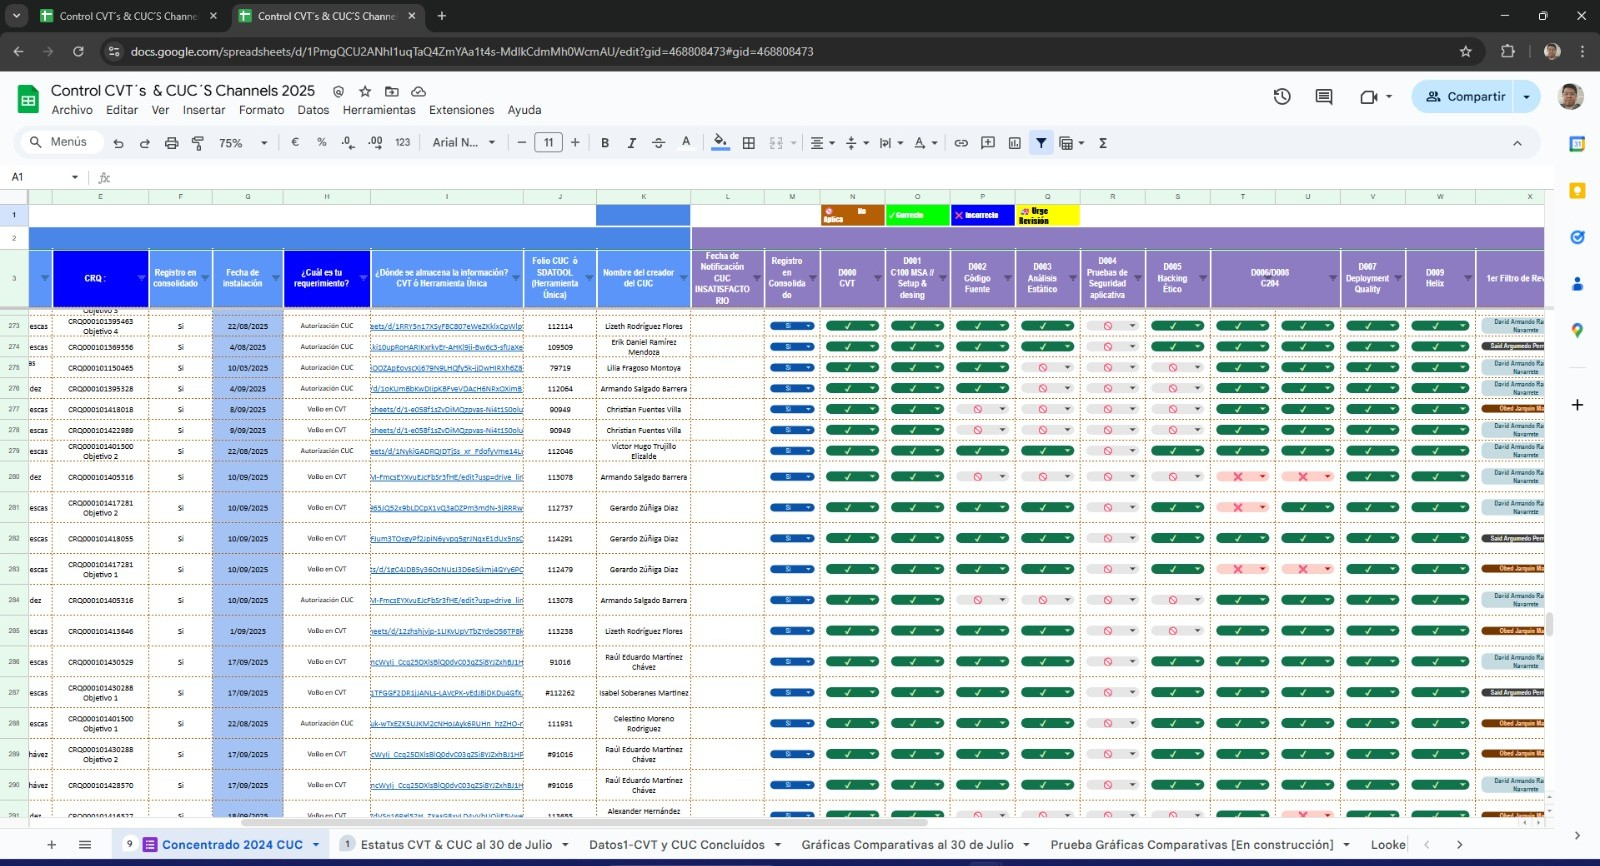
\includegraphics[width=0.9\textwidth]{E3_R1_SPDS}
    \caption{Base de datos consolidada empleada para el control y seguimiento de los procesos analizados, utilizada como fuente principal para la generación de métricas y reportes operativos.}
    \label{fig:base_datos_consolidada}
\end{figure}

\begin{figure}[H]
    \centering
    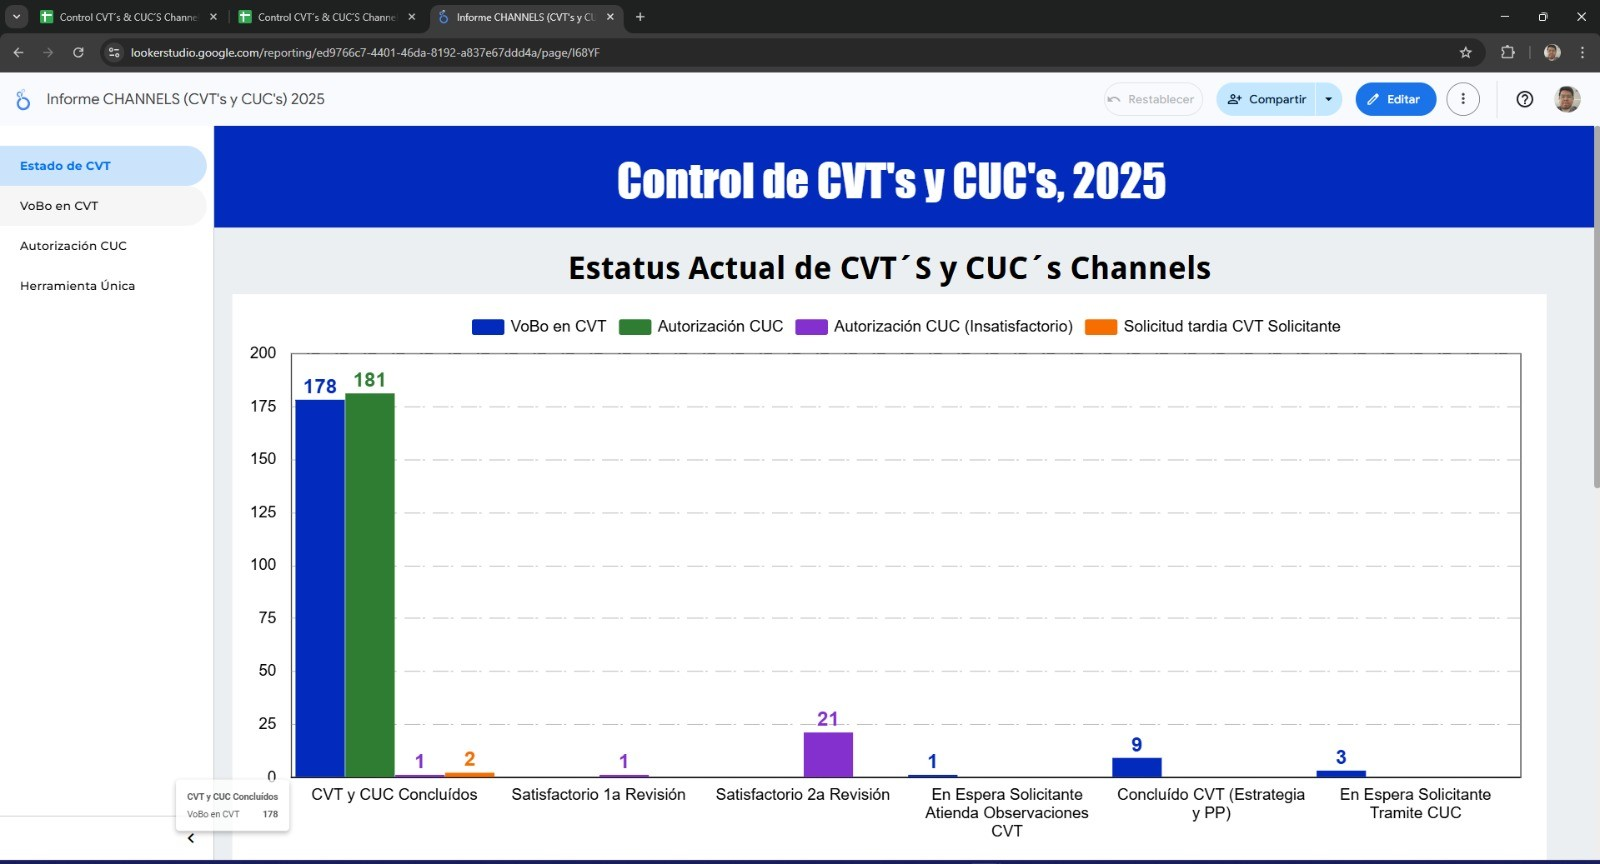
\includegraphics[width=0.9\textwidth]{E3_R1_LS_1}
    \caption{Visualización del estatus actual de los procesos analizados, mostrando la distribución de actividades concluidas, en revisión y en espera, utilizada para el seguimiento del avance operativo.}
    \label{fig:estatus_general_procesos}
\end{figure}

\begin{figure}[H]
    \centering
    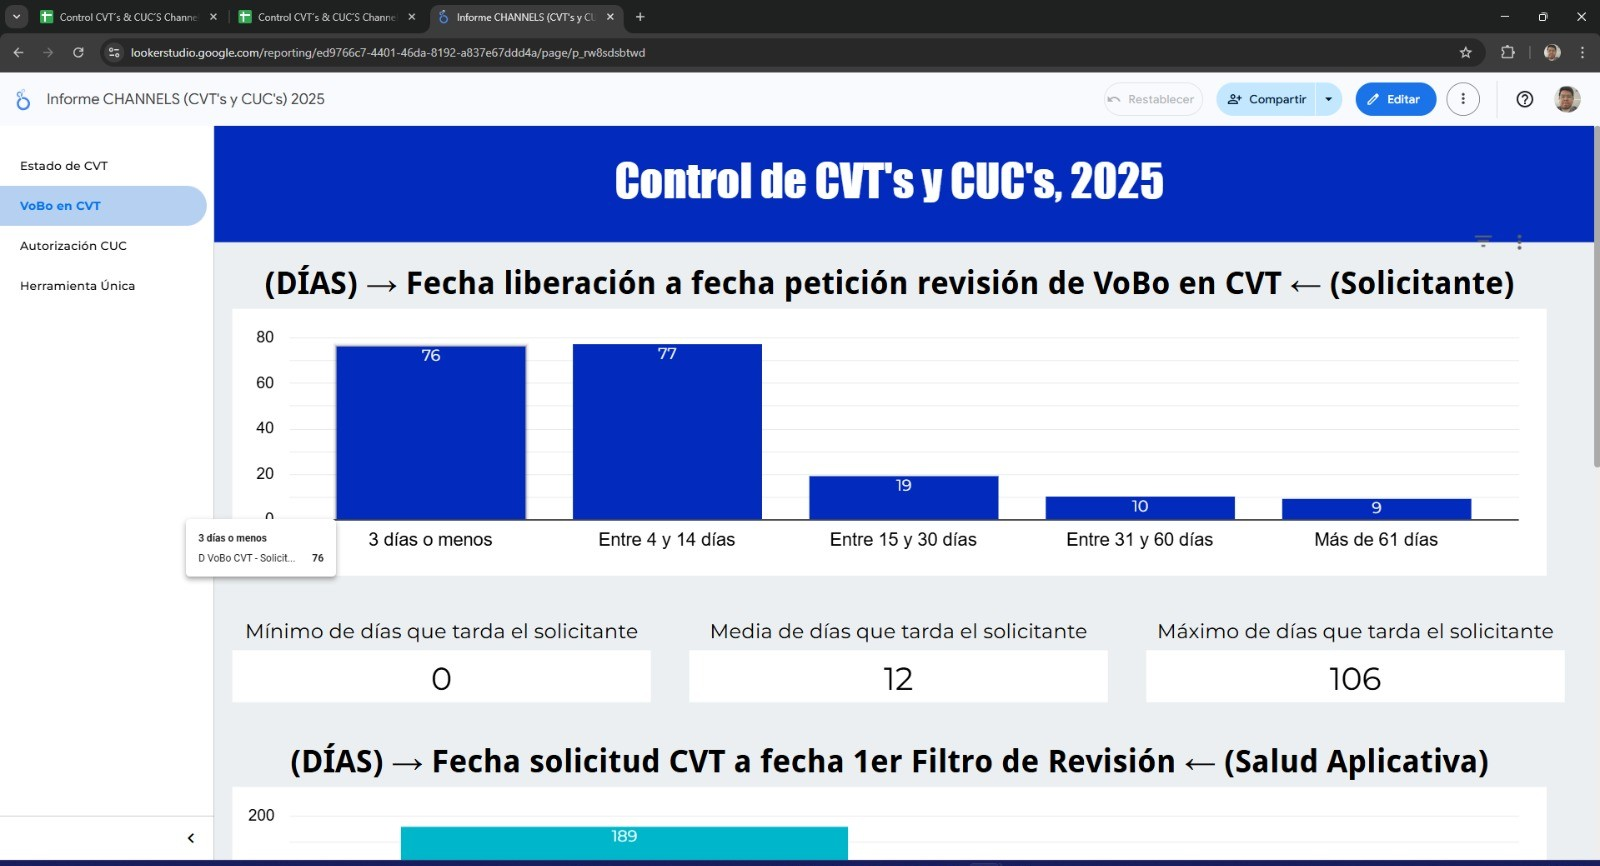
\includegraphics[width=0.9\textwidth]{E3_R1_LS_2}
    \caption{Distribución de los tiempos de atención clasificados por rangos de días, mostrando el intervalo transcurrido entre la liberación y la solicitud de revisión, utilizada para evaluar el comportamiento temporal del proceso.}
    \label{fig:tiempos_solicitante}
\end{figure}

\begin{figure}[H]
    \centering
    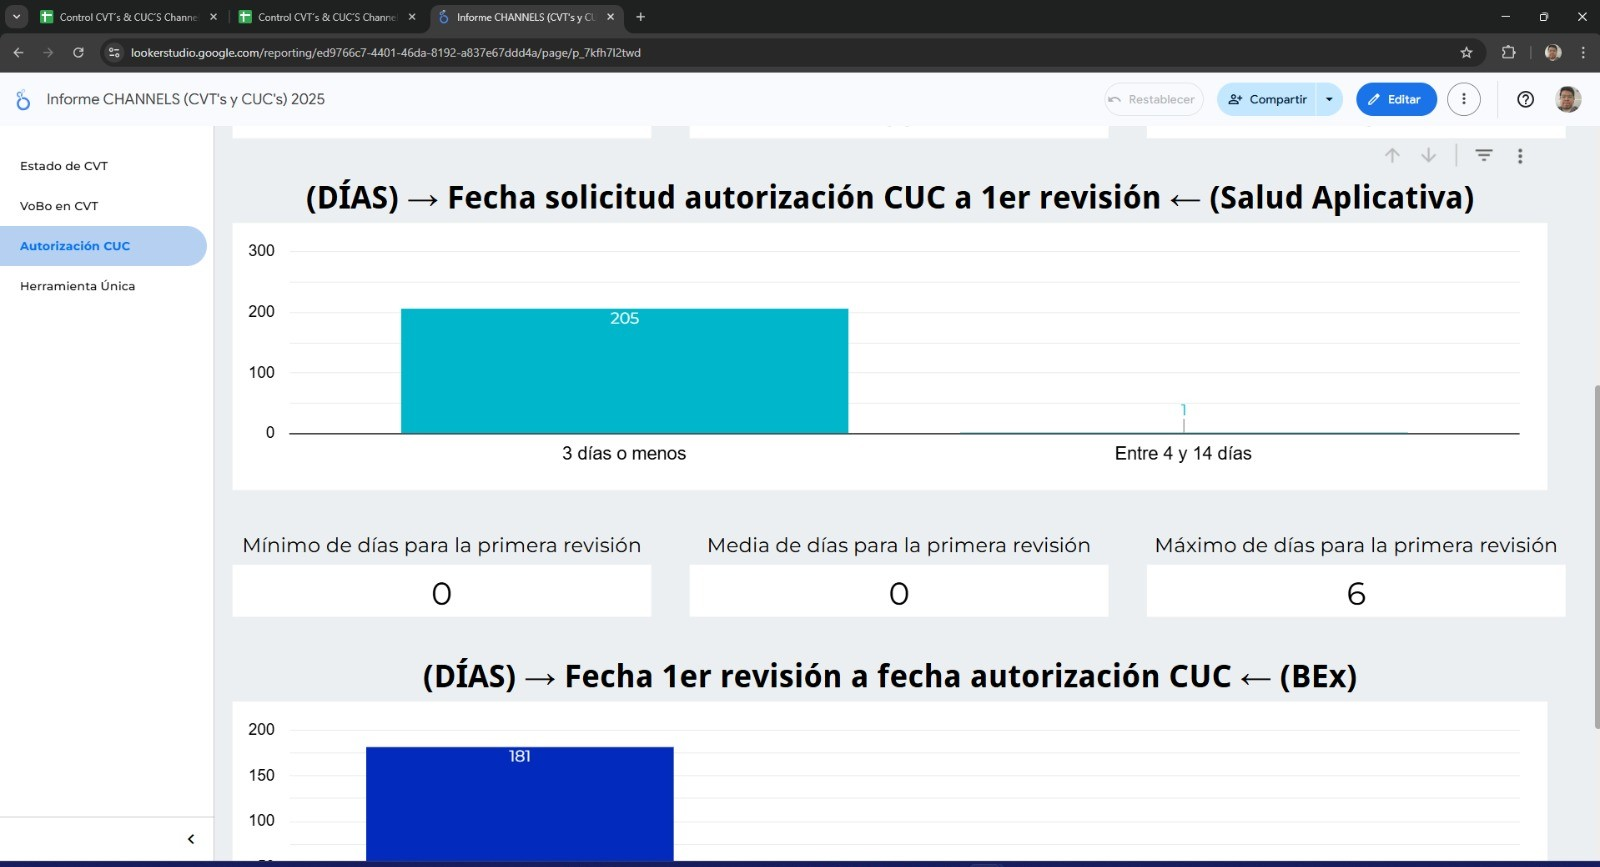
\includegraphics[width=0.9\textwidth]{E3_R1_LS_3}
    \caption{Distribución de los tiempos de atención entre la solicitud de autorización y la primera revisión, clasificados por rangos de días, utilizada para evaluar la eficiencia en una etapa intermedia del proceso.}
    \label{fig:tiempos_autorizacion_revision}
\end{figure}

\begin{figure}[H]
    \centering
    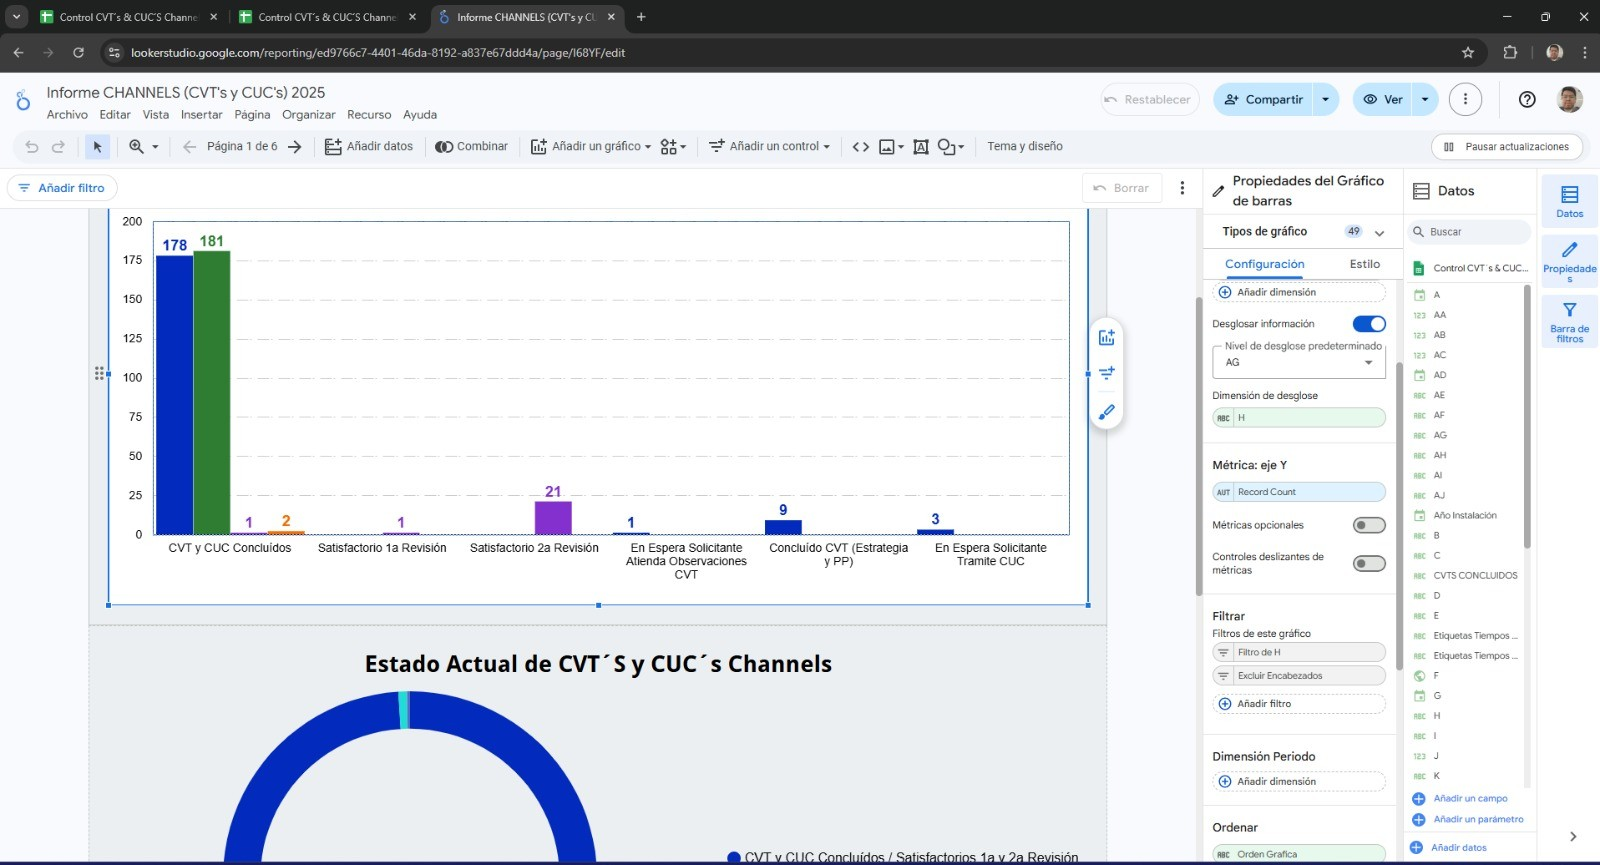
\includegraphics[width=0.9\textwidth]{E3_R1_ED1}
    \caption{Configuración del gráfico de barras utilizado para representar el estatus actual de los procesos, mostrando la selección de dimensiones, métricas y filtros aplicados para la visualización de resultados agregados.}
    \label{fig:config_grafico_estatus}
\end{figure}

\begin{figure}[H]
    \centering
    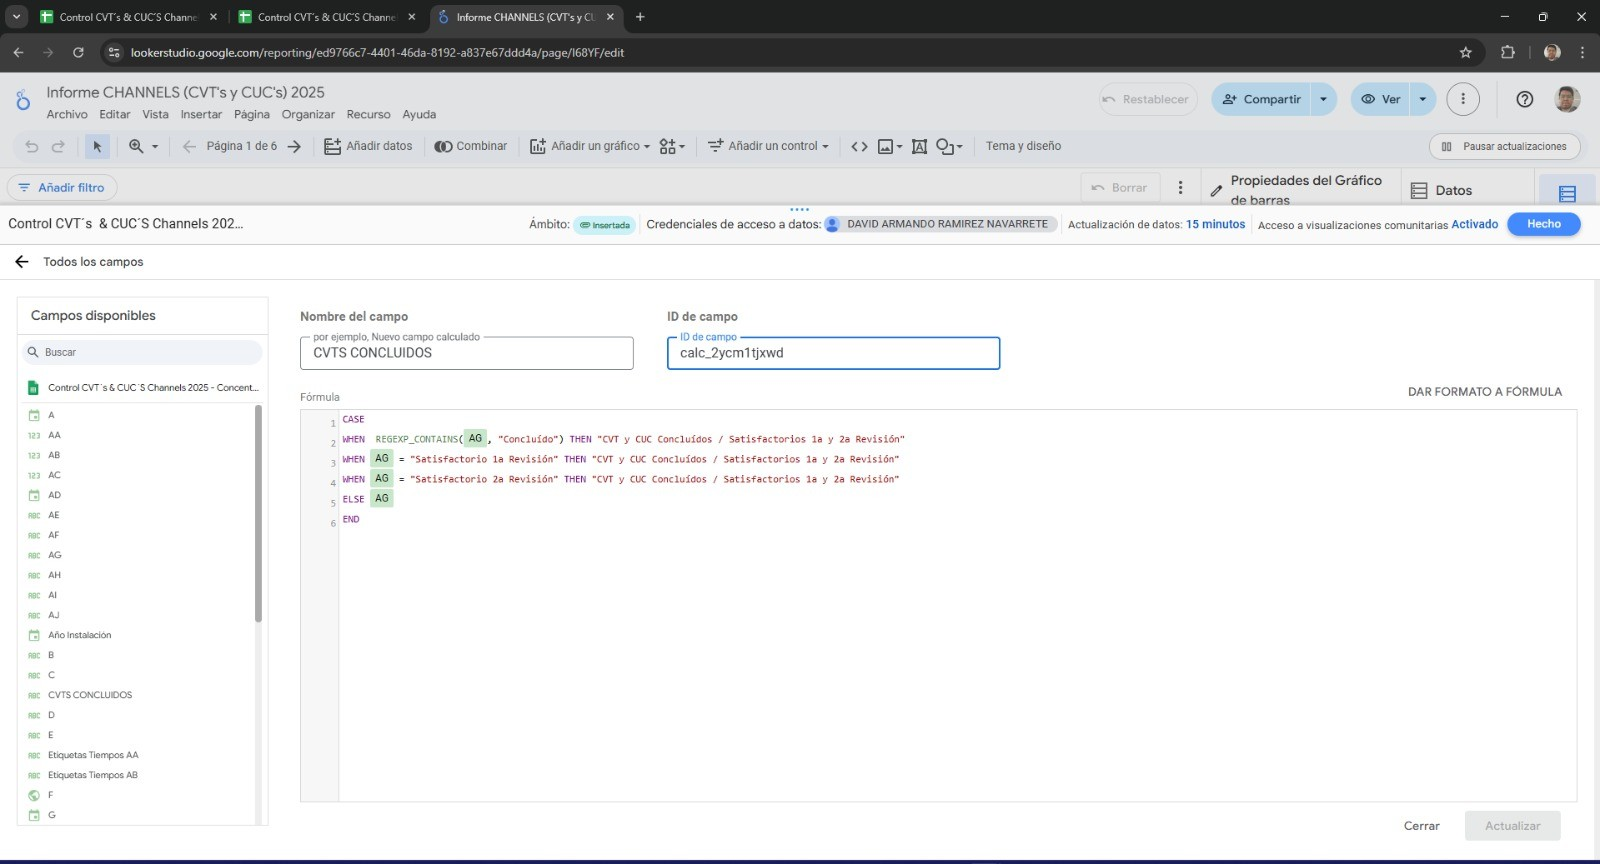
\includegraphics[width=0.9\textwidth]{E3_R1_ED2}
    \caption{Definición de un campo calculado para la agrupación de distintos estatus de los procesos en una categoría consolidada, mediante el uso de condiciones lógicas y expresiones regulares, con el fin de facilitar el análisis de resultados.}
    \label{fig:campo_calculado_estatus}
\end{figure}

\begin{figure}[H]
    \centering
    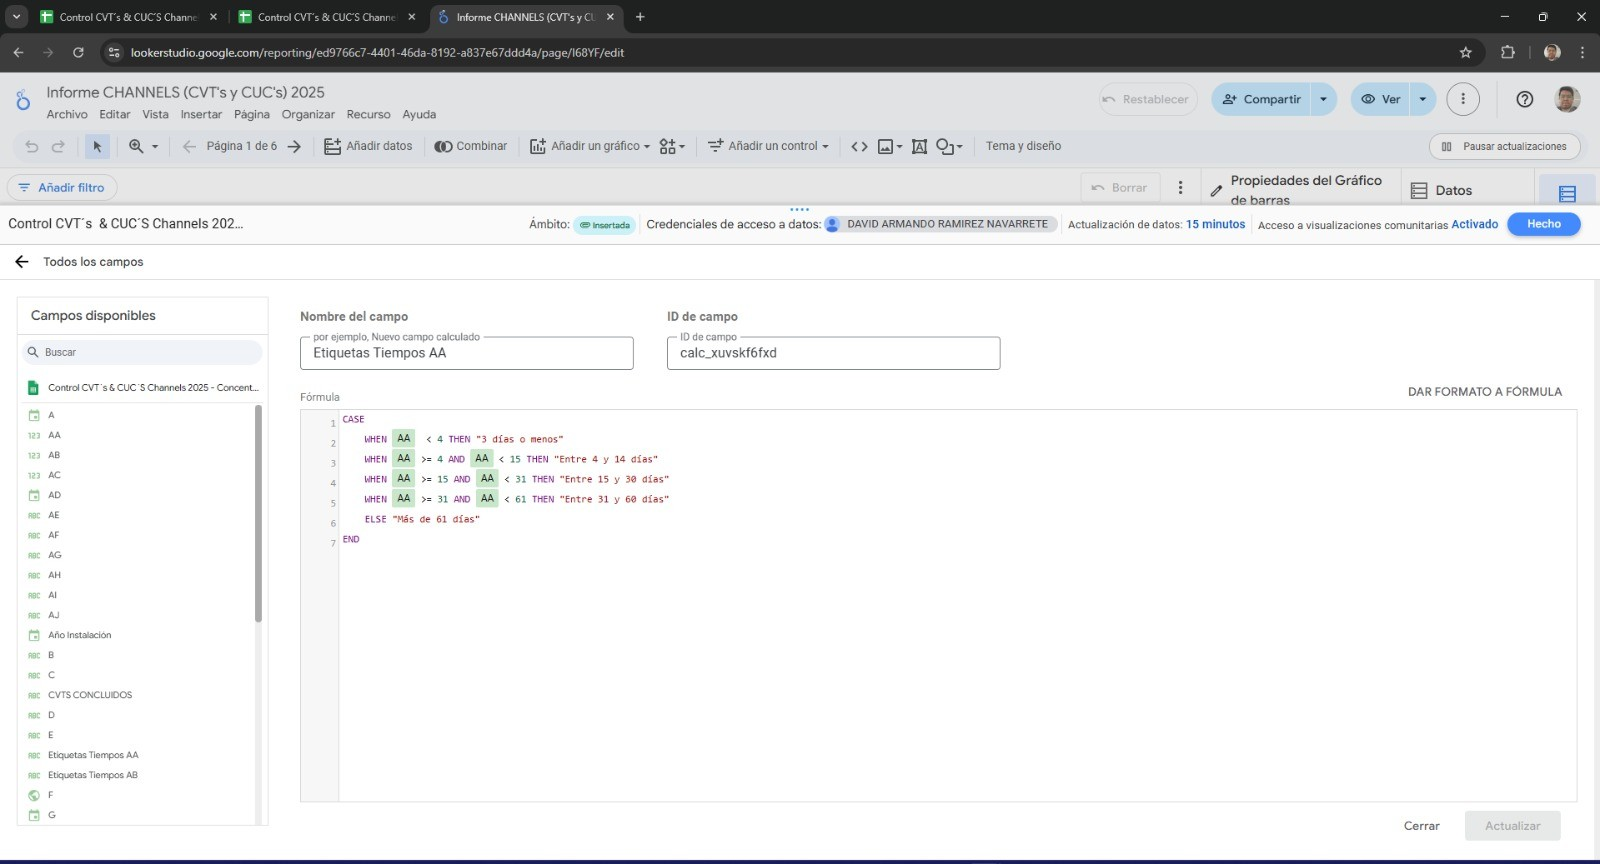
\includegraphics[width=0.9\textwidth]{E3_R1_ED3}
    \caption{Definición de un campo calculado para la clasificación de los tiempos de atención en rangos de días, mediante condiciones lógicas, con el objetivo de facilitar su análisis y visualización.}
    \label{fig:campo_calculado_tiempos}
\end{figure}

\begin{figure}[H]
    \centering
    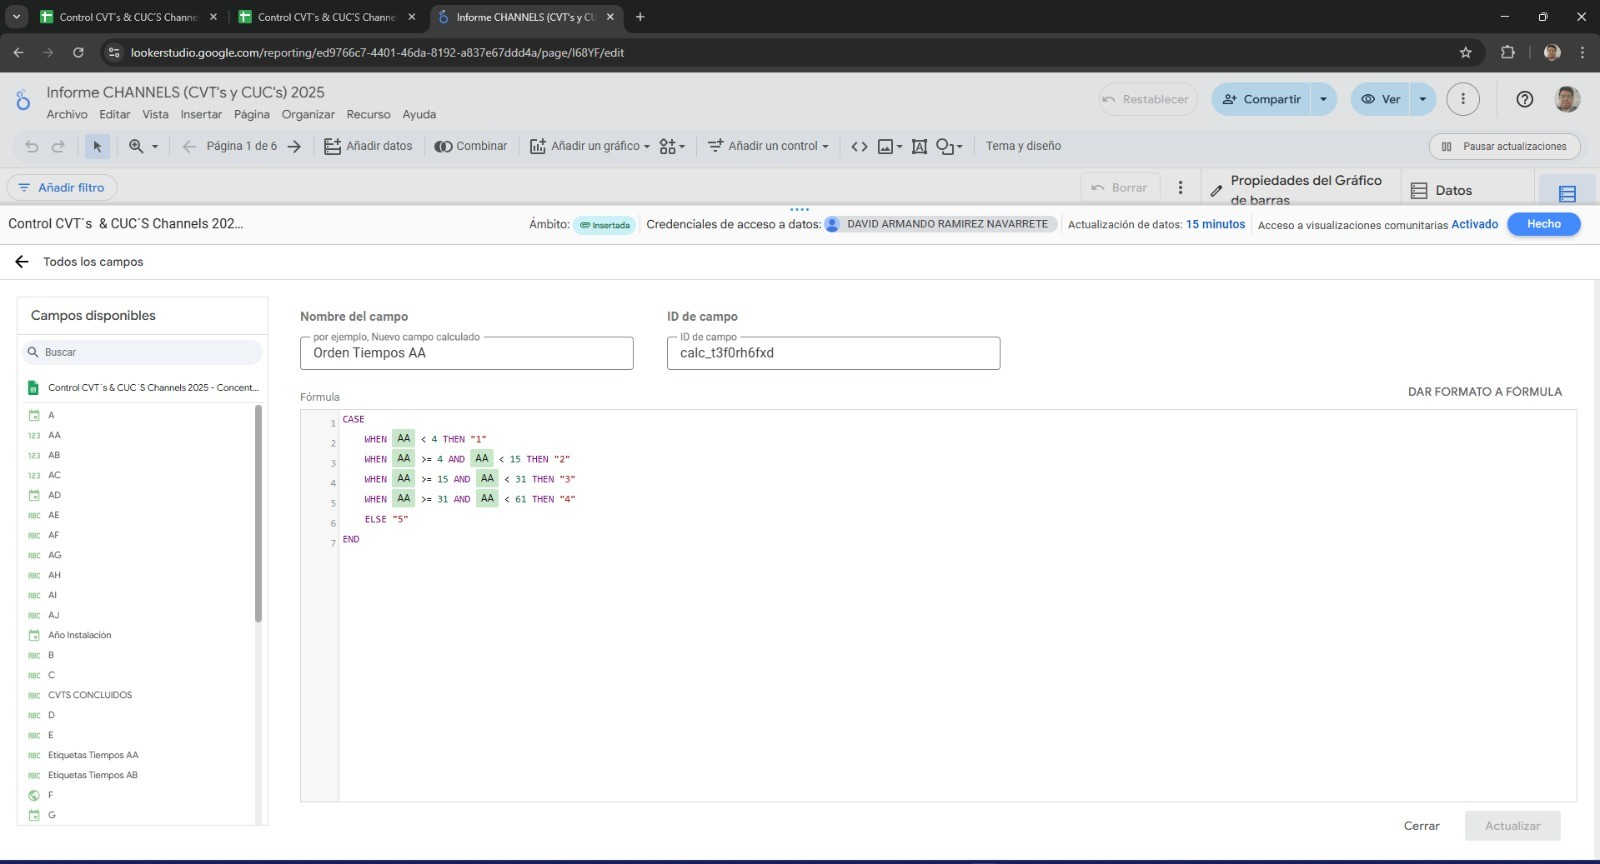
\includegraphics[width=0.9\textwidth]{E3_R1_ED4}
    \caption{Definición de un campo calculado auxiliar para establecer el orden lógico de los rangos de tiempo, utilizado para asegurar una correcta disposición de las categorías en las visualizaciones gráficas.}
    \label{fig:orden_tiempos}
\end{figure}

\begin{figure}[H]
    \centering
    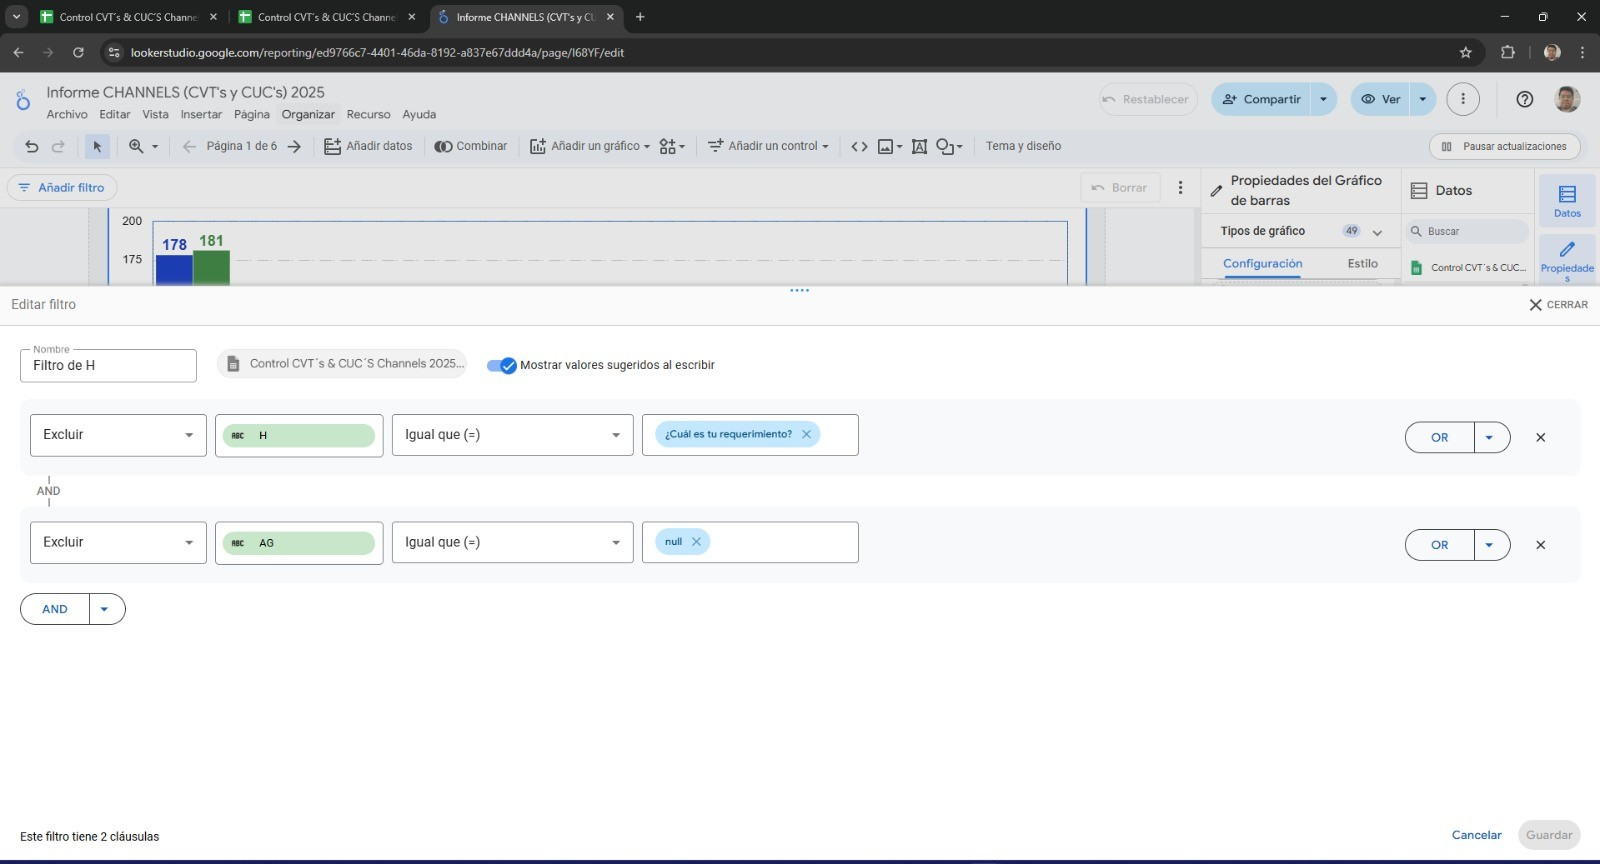
\includegraphics[width=0.9\textwidth]{E3_R1_ED5}
    \caption{Configuración de filtros para la exclusión de registros no relevantes y valores nulos, aplicada con el objetivo de asegurar la calidad y consistencia de la información utilizada en el análisis.}
    \label{fig:filtros_calidad_datos}
\end{figure}

\begin{figure}[H]
    \centering
    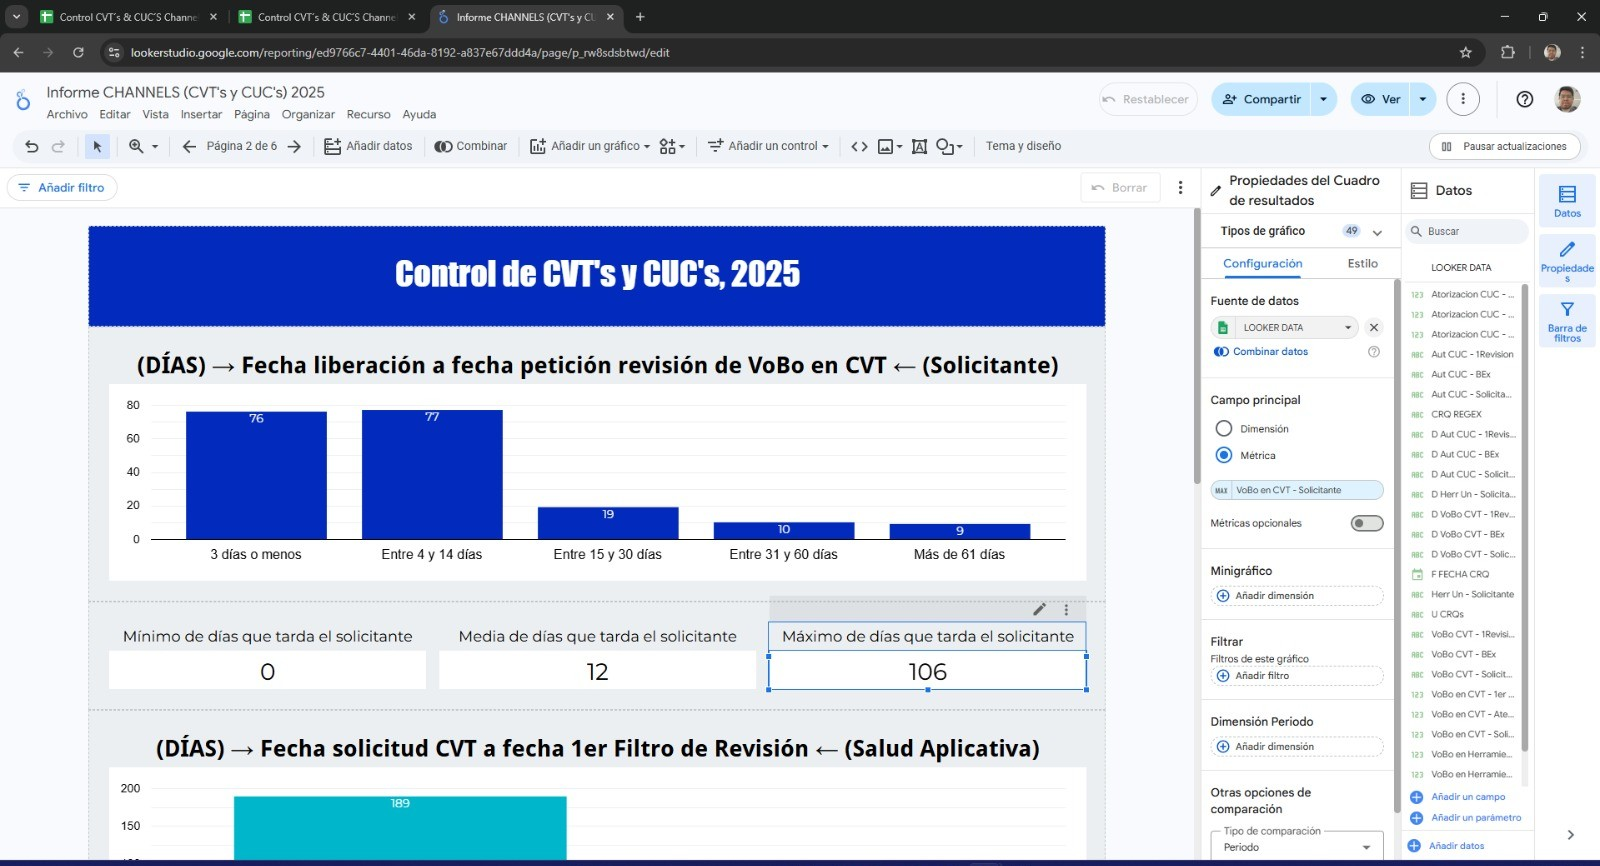
\includegraphics[width=0.9\textwidth]{E3_R1_ED6}
    \caption{Visualización final de los indicadores de tiempo y métricas agregadas, utilizada para el análisis del desempeño operativo y la validación de los resultados obtenidos a partir de los campos calculados.}
    \label{fig:visualizacion_final_tiempos}
\end{figure}

\begin{figure}[H]
    \centering
    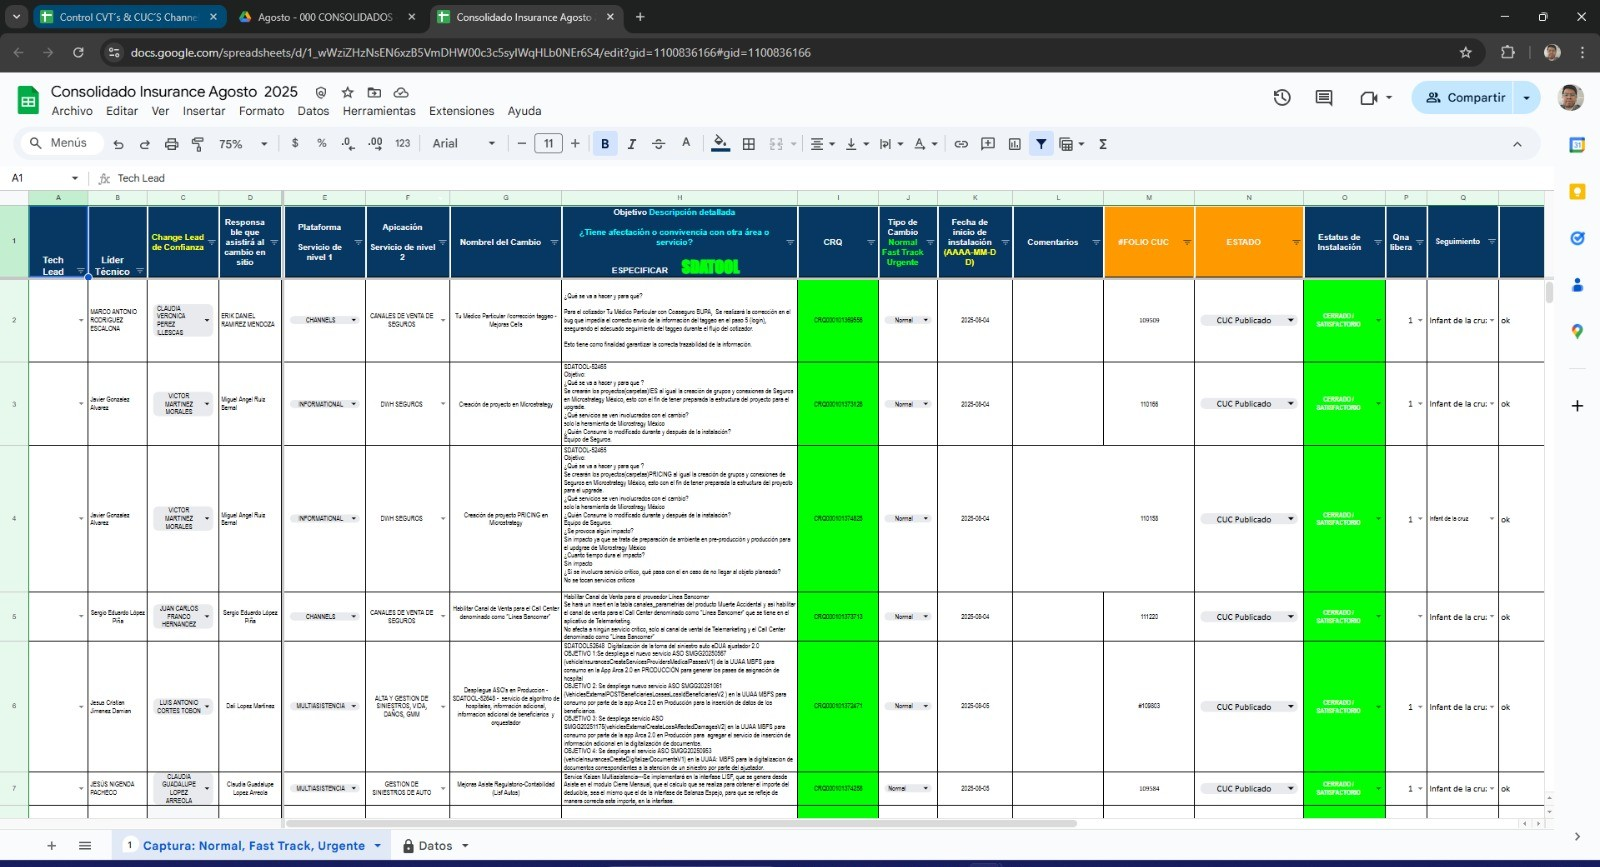
\includegraphics[width=0.95\textwidth]{E3_R2_SPDS1}
    \caption{Hoja de cálculo utilizada como fuente de datos consolidada para el análisis de procesos operativos, en la cual se registran identificadores, fechas, estatus y resultados, sirviendo como base para la generación de métricas y reportes.}
    \label{fig:base_datos_consolidada_cambios}
\end{figure}

\begin{figure}[H]
    \centering
    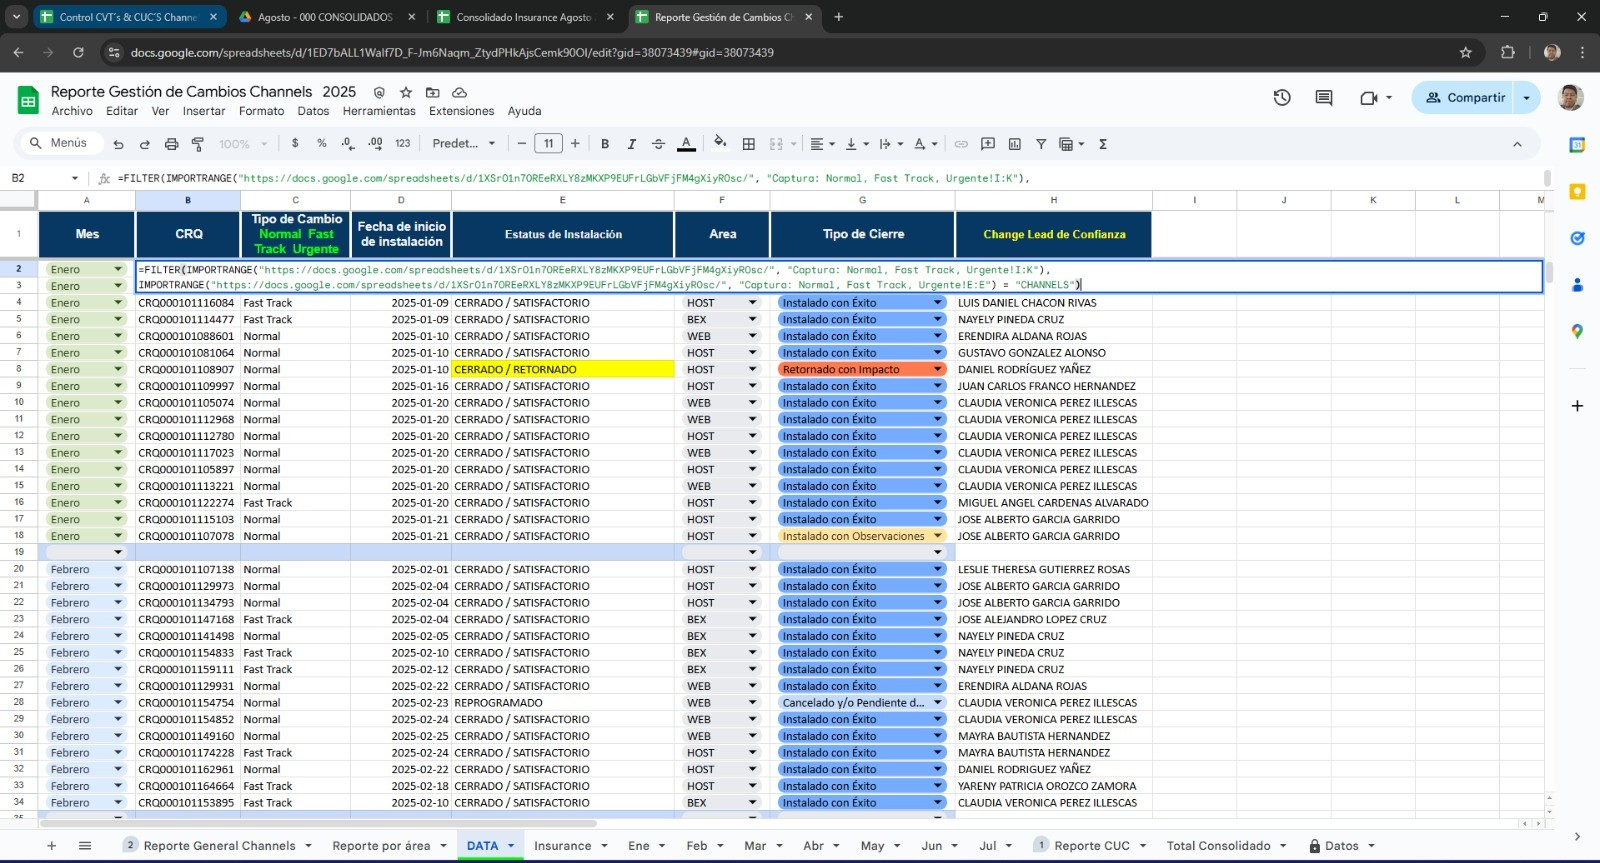
\includegraphics[width=0.95\textwidth]{E3_R2_SPDS2}
    \caption{Hoja de cálculo intermedia utilizada para la consolidación automática de información mediante funciones de importación y filtrado, permitiendo integrar datos de múltiples fuentes para su posterior análisis y generación de reportes.}
    \label{fig:integracion_datos_import}
\end{figure}

\begin{figure}[H]
    \centering
    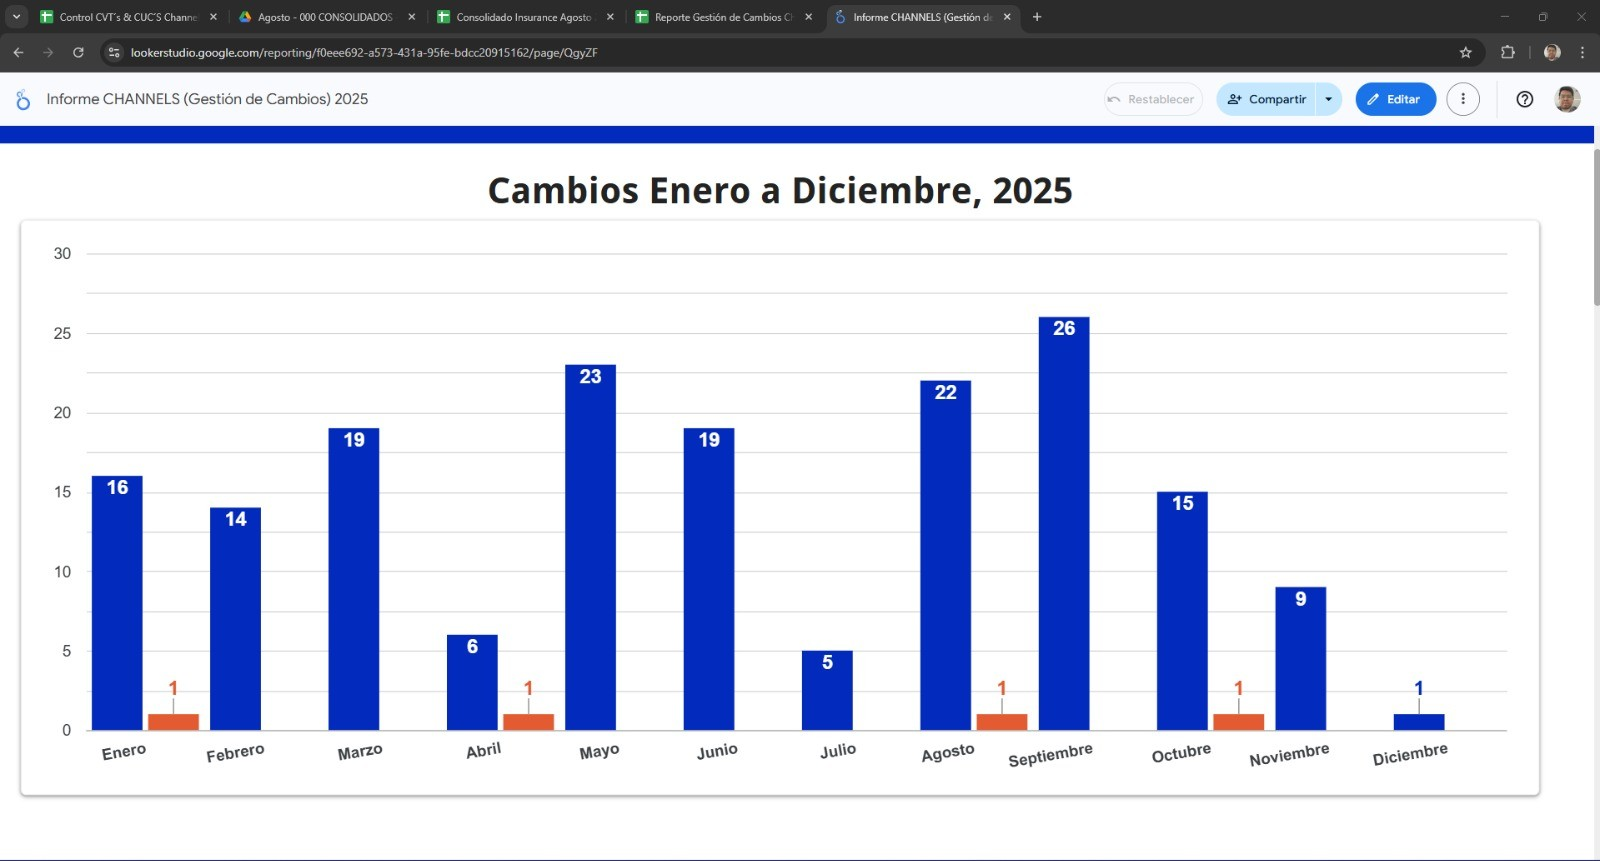
\includegraphics[width=0.95\textwidth]{E3_R2_LS1}
    \caption{Distribución mensual del volumen de cambios gestionados durante el año, utilizada para identificar patrones de carga operativa y variaciones en la demanda a lo largo del periodo analizado.}
    \label{fig:cambios_mensuales}
\end{figure}

\begin{figure}[H]
    \centering
    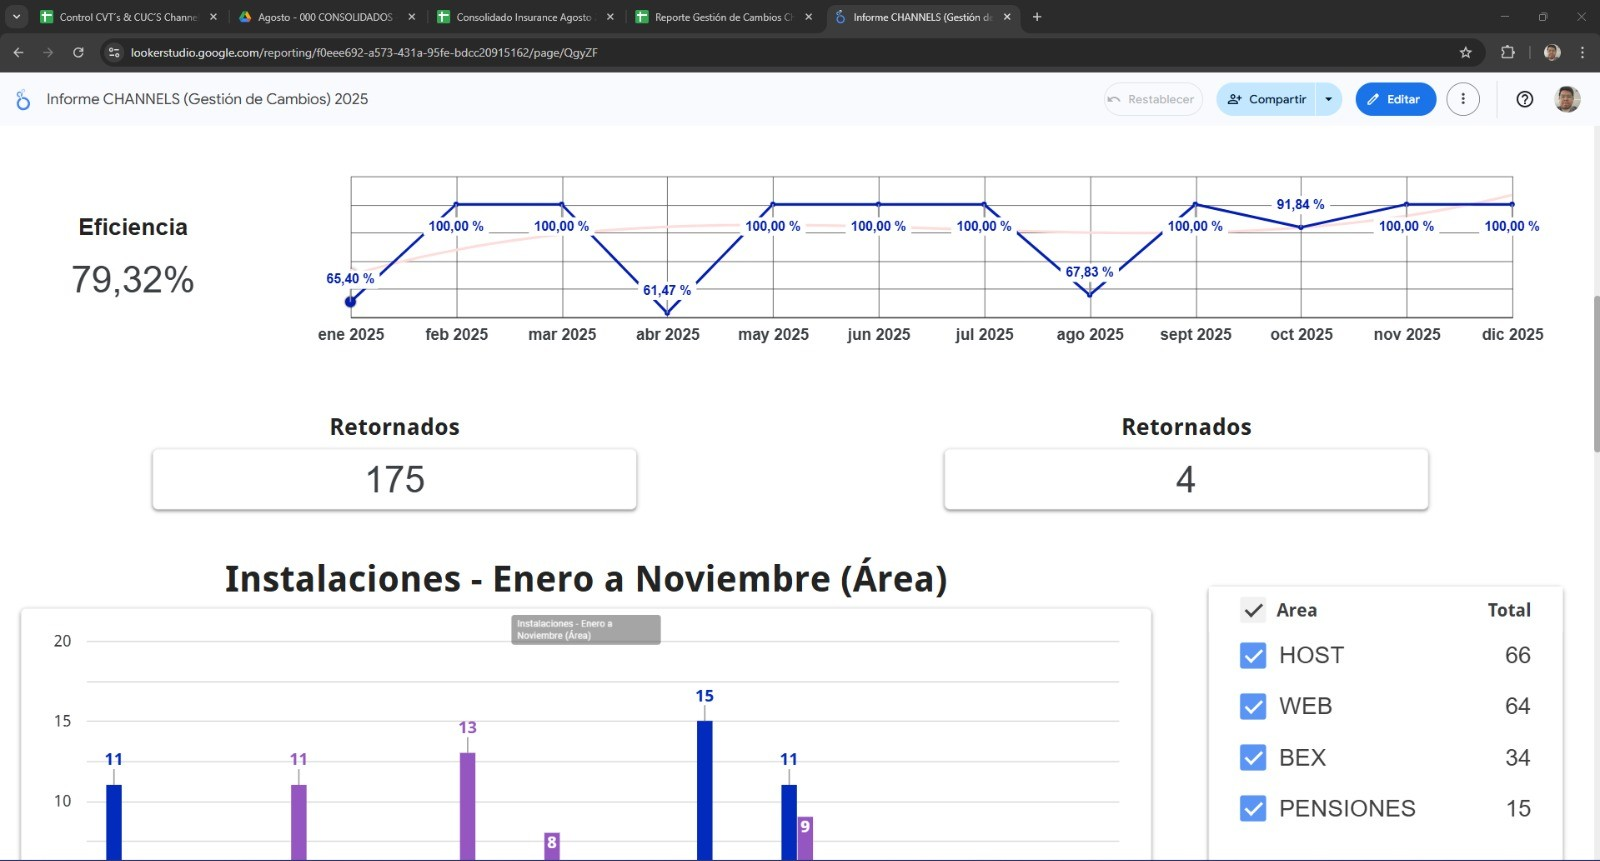
\includegraphics[width=0.95\textwidth]{E3_R2_LS2}
    \caption{Indicadores de eficiencia operativa y número de cambios retornados a lo largo del periodo analizado, empleados para evaluar el desempeño del proceso y su estabilidad en el tiempo.}
    \label{fig:eficiencia_operativa}
\end{figure}

\begin{figure}[H]
    \centering
    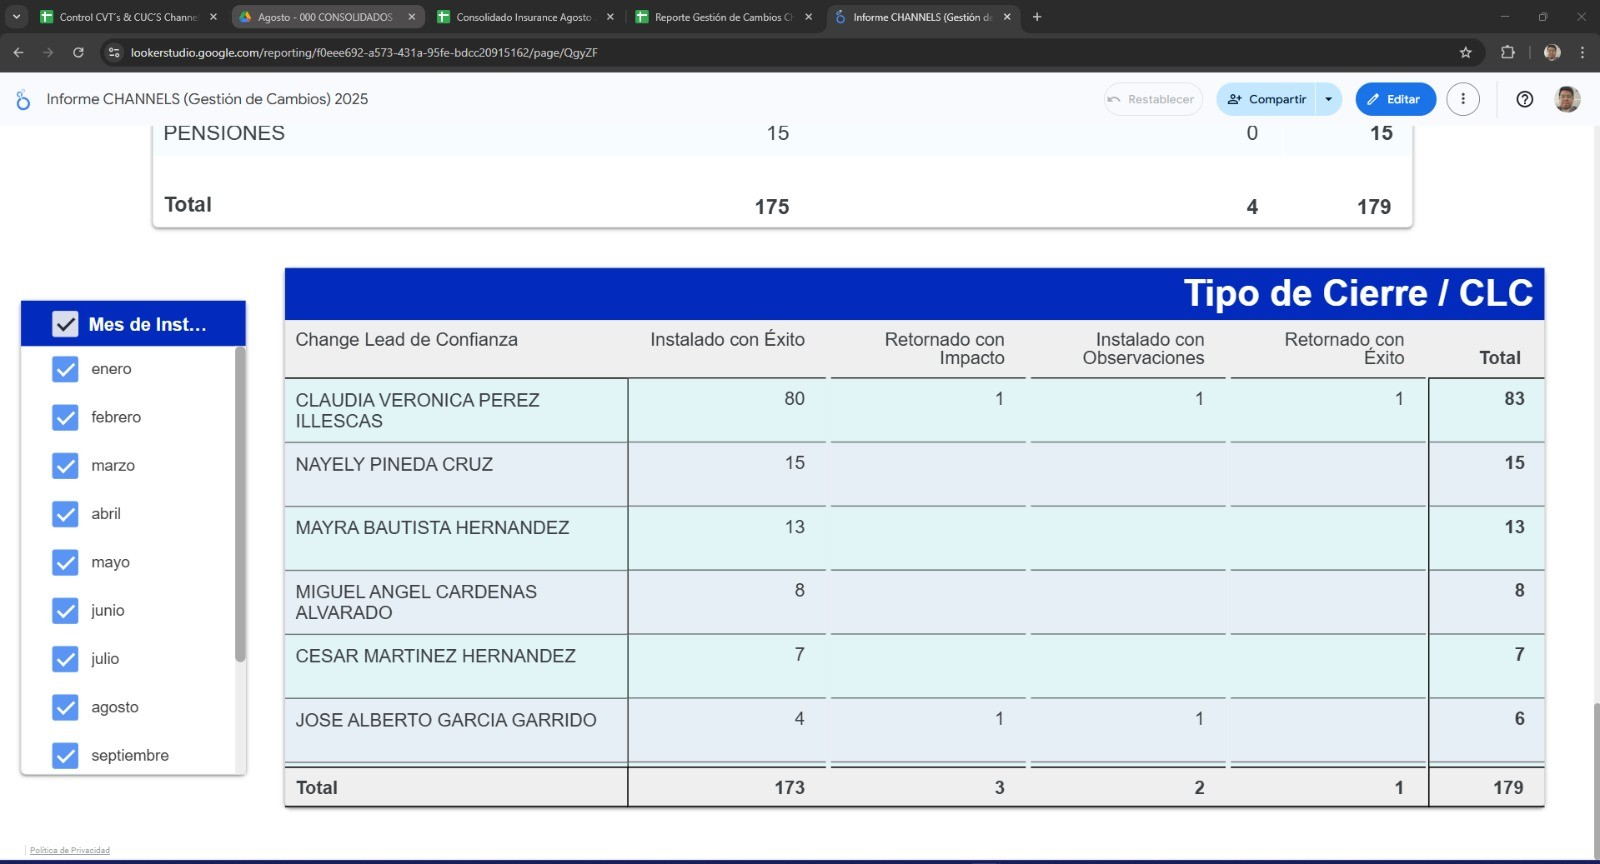
\includegraphics[width=0.95\textwidth]{E3_R2_LS3}
    \caption{Distribución de los cambios gestionados según el tipo de cierre y su asignación por responsable, utilizada para evaluar la efectividad del proceso y la calidad de los resultados obtenidos.}
    \label{fig:tipo_cierre_responsable}
\end{figure}

\begin{figure}[H]
    \centering
    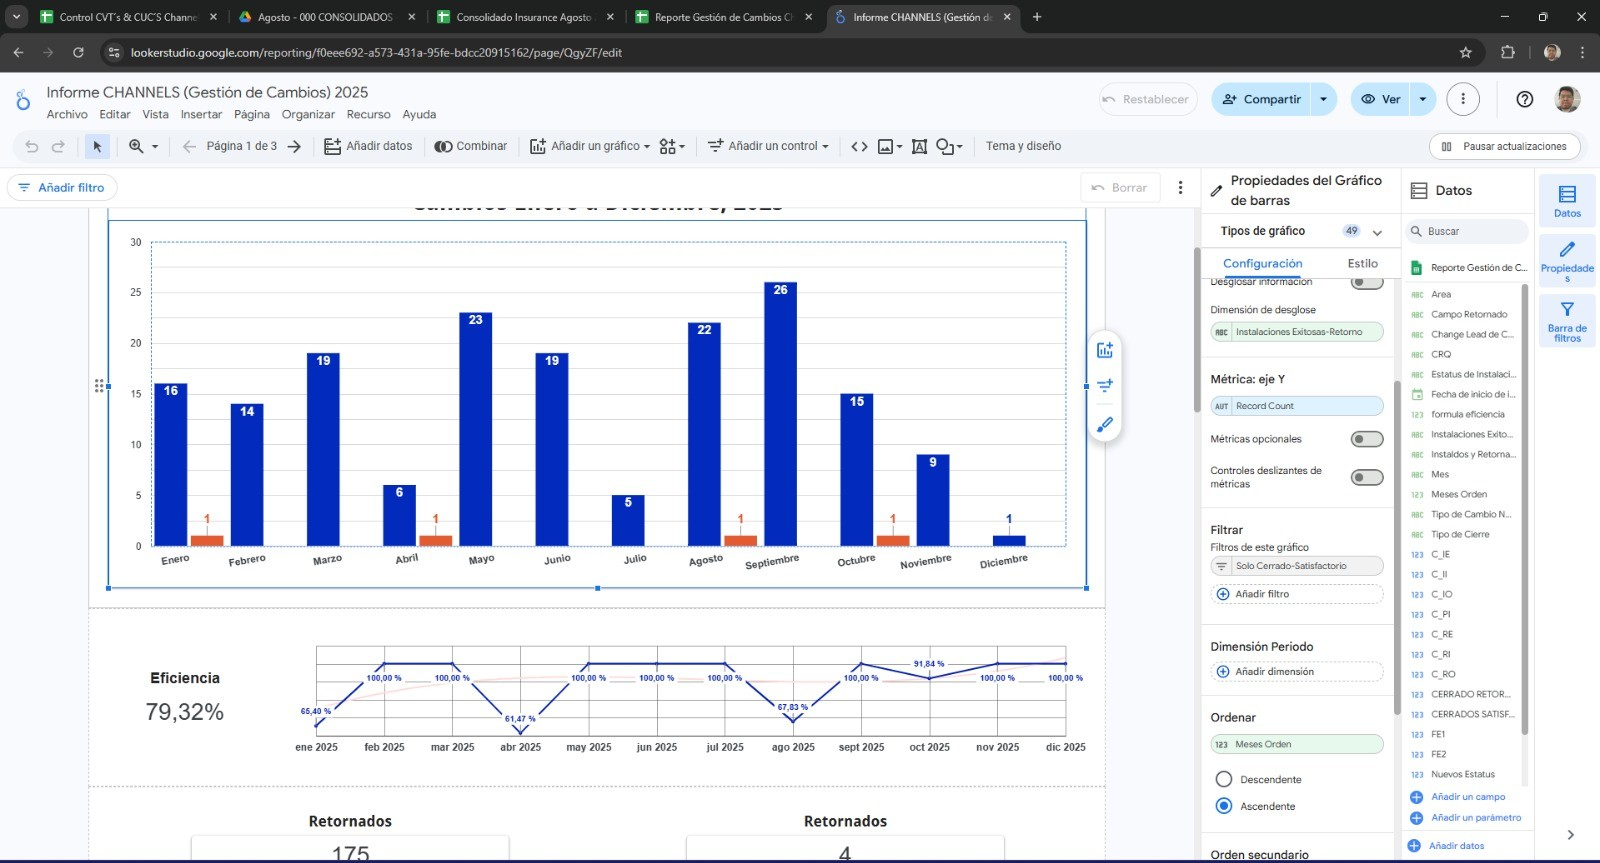
\includegraphics[width=0.95\textwidth]{E3_R2_ED1}
    \caption{Configuración del gráfico de barras utilizado para analizar la distribución mensual de los cambios gestionados, mostrando la selección de dimensiones temporales, métricas y criterios de filtrado aplicados.}
    \label{fig:config_cambios_mensuales}
\end{figure}

\begin{figure}[H]
    \centering
    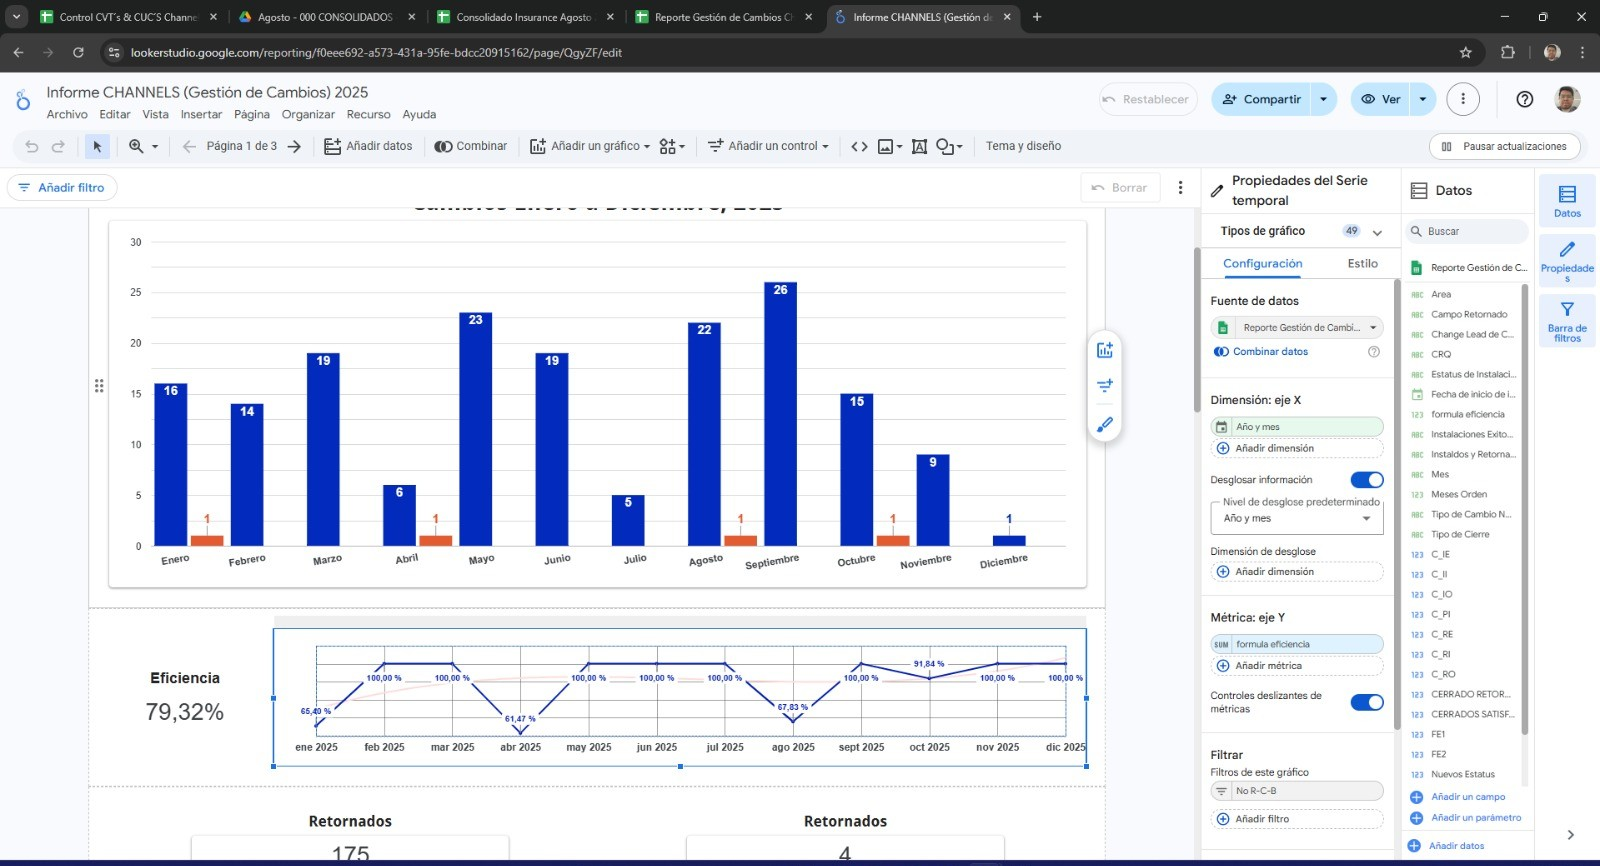
\includegraphics[width=0.95\textwidth]{E3_R2_ED2}
    \caption{Configuración de la serie temporal empleada para visualizar la evolución de la eficiencia operativa a lo largo del periodo analizado, a partir de métricas calculadas y dimensiones temporales.}
    \label{fig:config_eficiencia_temporal}
\end{figure}

\begin{figure}[H]
    \centering
    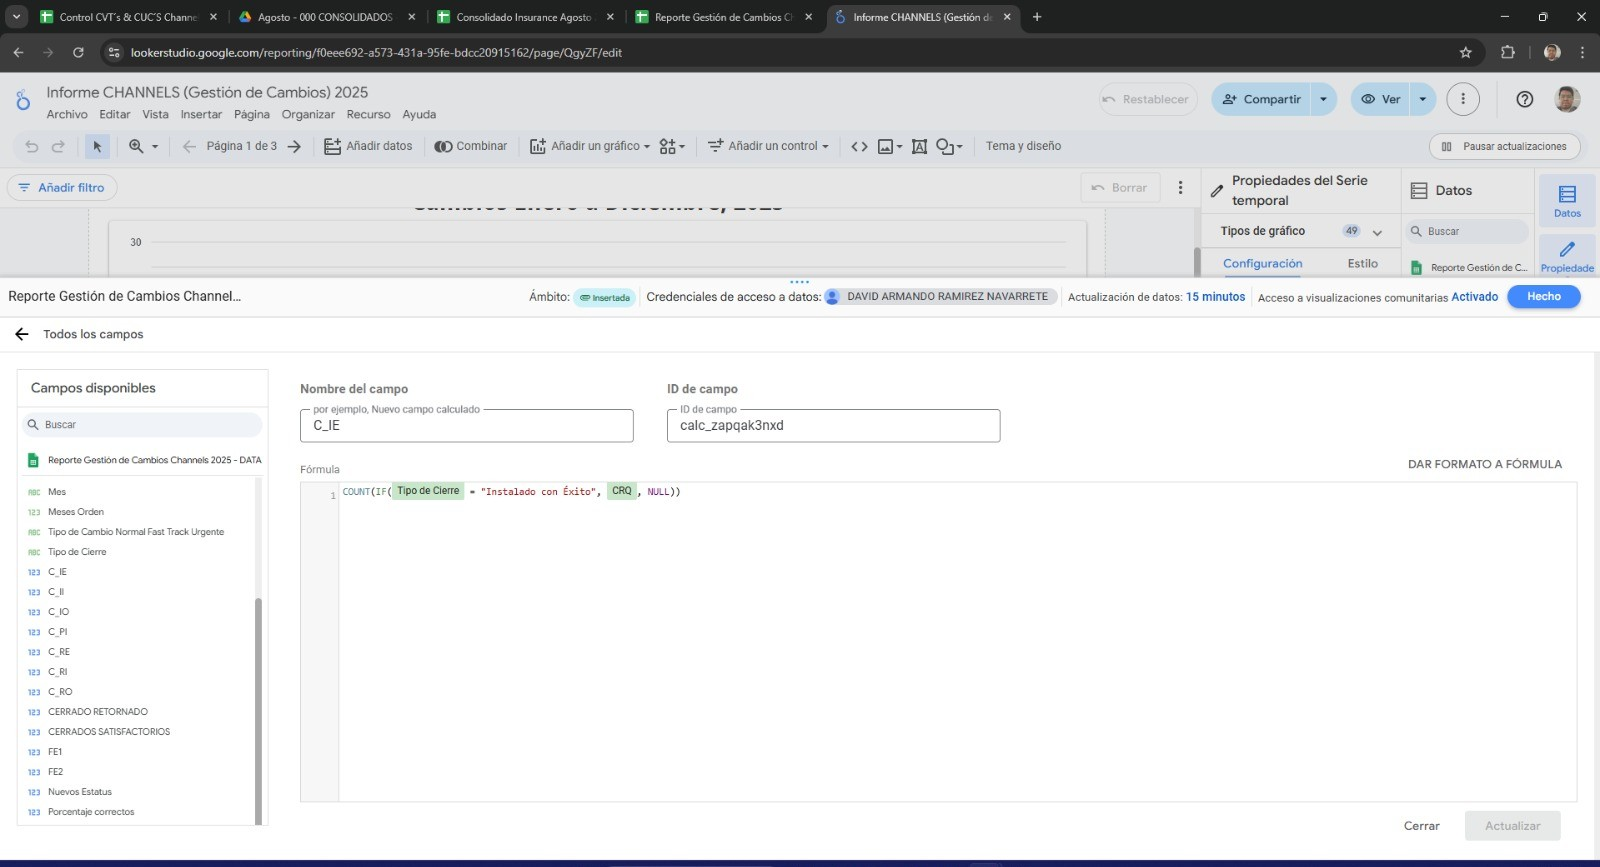
\includegraphics[width=0.9\textwidth]{E3_R2_ED3}
    \caption{Definición de un campo calculado para el conteo de cambios con cierre exitoso, mediante el uso de condiciones lógicas, con el fin de generar métricas específicas para el análisis de desempeño.}
    \label{fig:campo_instalaciones_exitosas}
\end{figure}

\begin{figure}[H]
    \centering
    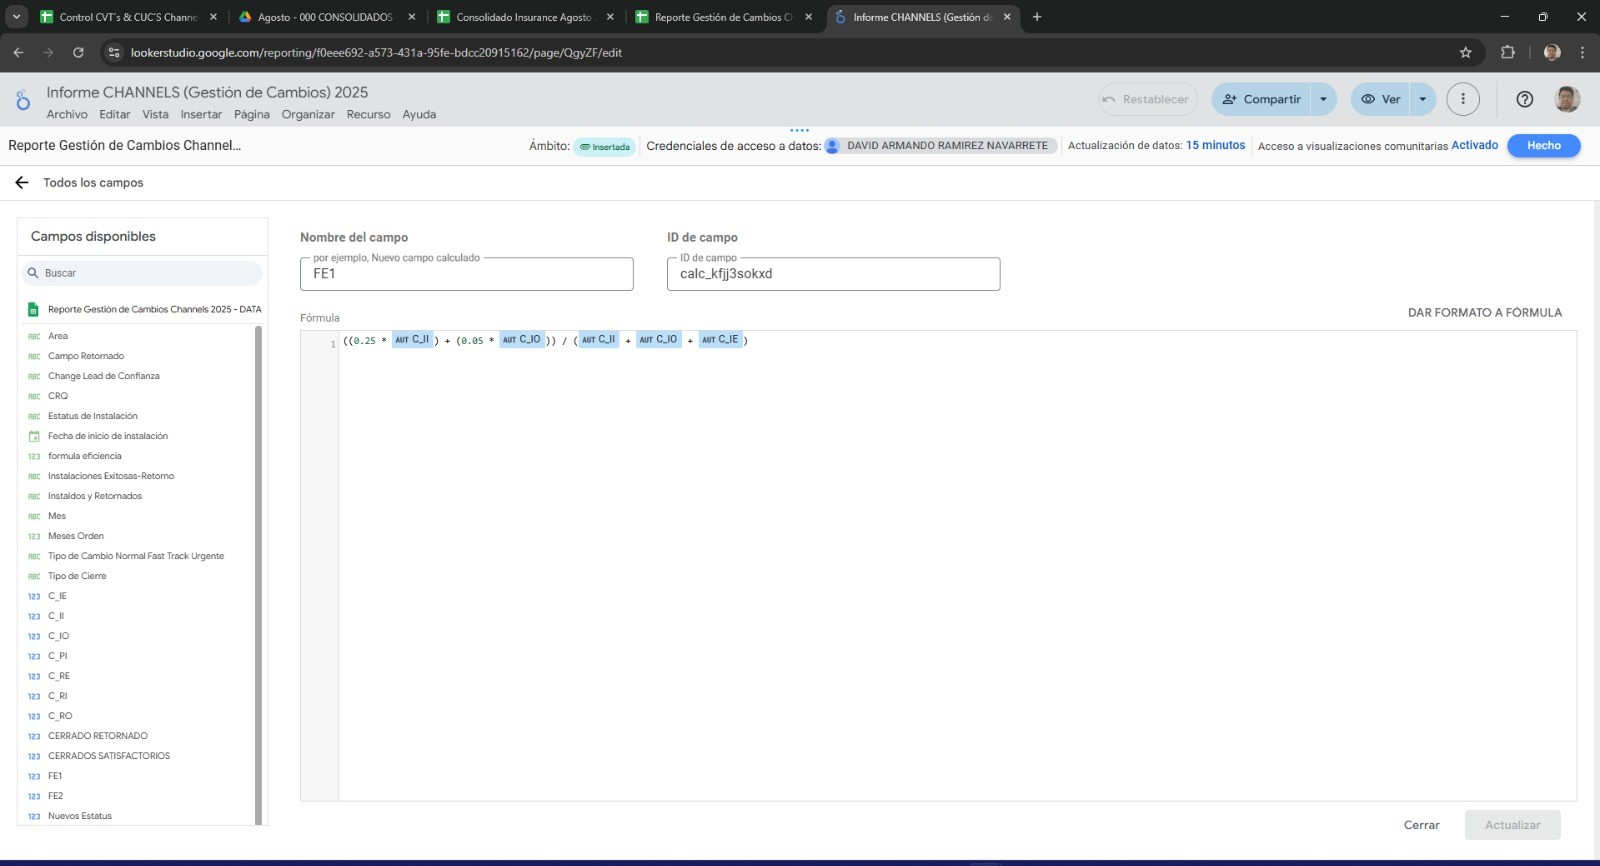
\includegraphics[width=0.9\textwidth]{E3_R2_ED4}
    \caption{Definición de una métrica intermedia utilizada como componente para el cálculo de eficiencia, integrando distintos tipos de cierre mediante una fórmula ponderada.}
    \label{fig:metrica_intermedia_fe1}
\end{figure}

\begin{figure}[H]
    \centering
    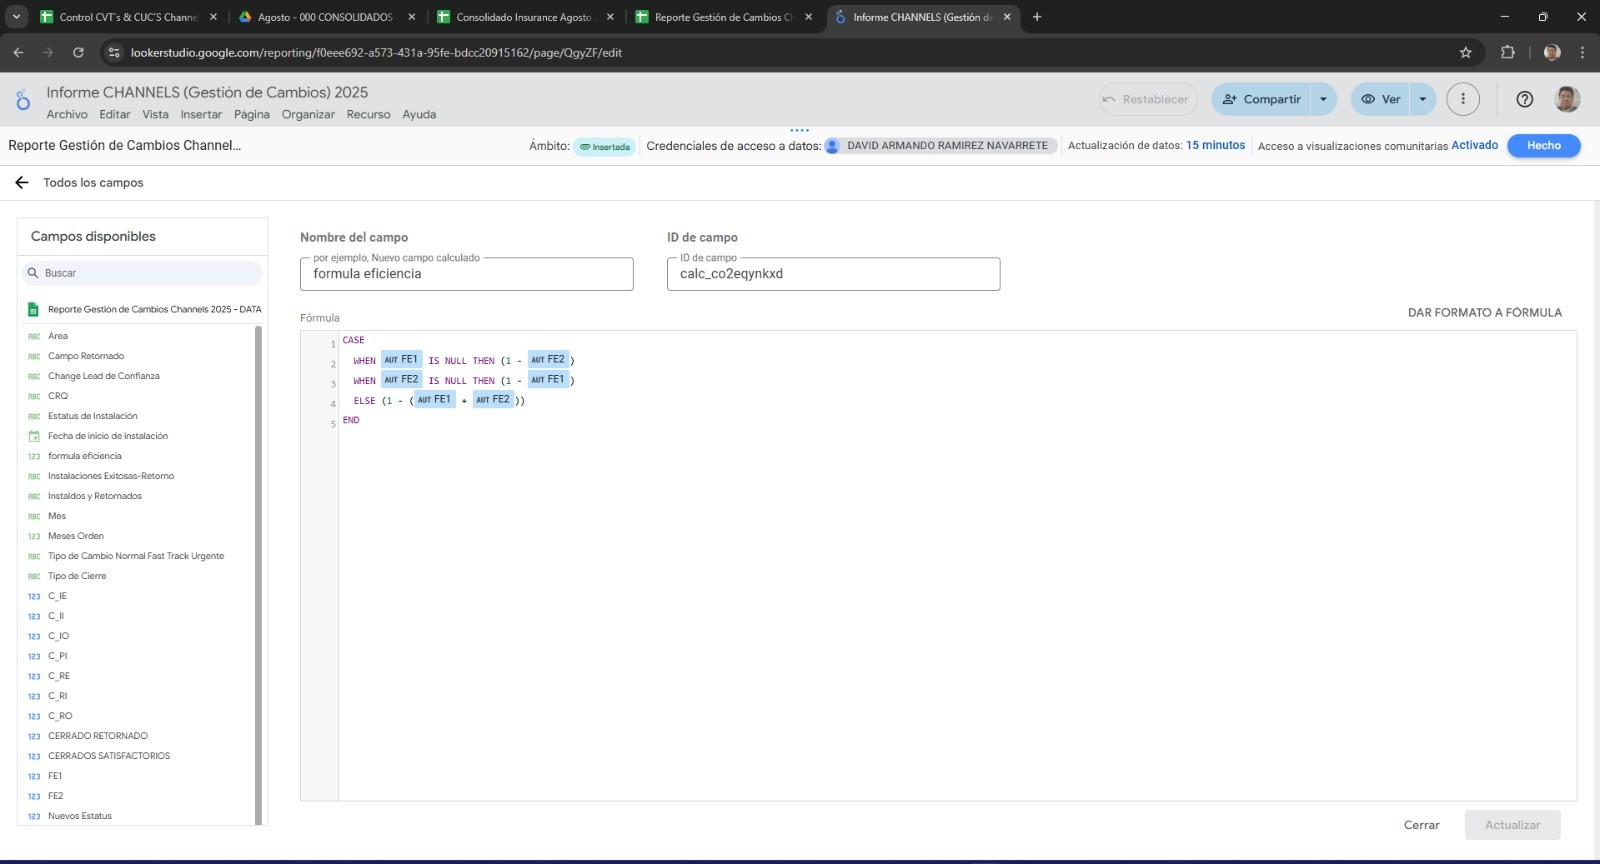
\includegraphics[width=0.9\textwidth]{E3_R2_ED5}
    \caption{Definición de la fórmula de eficiencia operativa mediante campos calculados, considerando distintos escenarios de datos nulos y combinando métricas parciales para obtener un indicador global de desempeño.}
    \label{fig:formula_eficiencia}
\end{figure}

\end{document}

